\section{Results}
\begin{frame}
  \frametitle{Results of the optimised program}
  \begin{figure}[h]
    \centering
    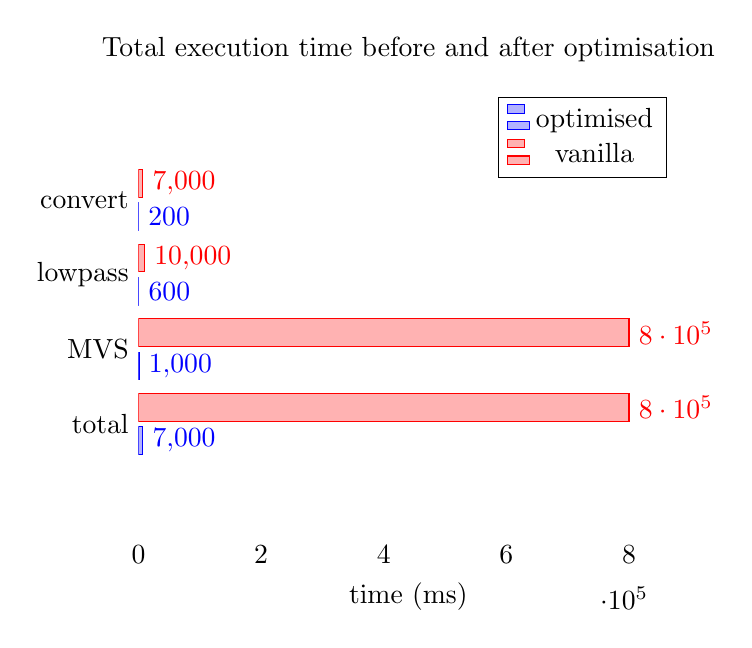
\begin{tikzpicture}
      \begin{axis}[
        title=Total execution time before and after optimisation,
        xbar, xmin=0,
        enlarge y limits=0.5,
        y axis line style={opacity=0},
        tickwidth=0pt,
        xlabel={time (ms)},
        ytick=data,
        symbolic y coords = {total, MVS, lowpass, convert},
        nodes near coords
        ]
        \addplot coordinates {(200,convert) (600,lowpass)
          (1000,MVS) (7000,total)};
        \addplot coordinates {(7000,convert) (10000,lowpass)
          (800000,MVS) (800000,total)};
        \legend{optimised, vanilla}
      \end{axis}
    \end{tikzpicture}
  \end{figure}
\end{frame}

\begin{frame}[fragile]
  \frametitle{Correctness of the optimised program}
\begin{verbatim}
      ...
>>  Comparing frame 2
      Check for frame_ycbcr.Y frames OK
      Check for frame_ycbcr.Cb frames OK
      Check for frame_ycbcr.Cr frames OK
      Check for frame_ycbcr_lowpass.Y frames OK
      Check for frame_ycbcr_lowpass.Cb frames OK
      Check for frame_ycbcr_lowpass.Cr frames OK
      Check for frame_downsampled.Y frames OK
      Check for frame_downsampled.Cb frames OK
      Check for frame_downsampled.Cr frames OK
      Check for frame_dct.Y frames OK
      Check for frame_dct.Cb frames OK
      ...
\end{verbatim}
\end{frame}

%%% Local Variables:
%%% mode: latex
%%% TeX-master: "presentation"
%%% End:
